\pagestyle{empty}
\cleardoublepage
\pagestyle{fancy}

\selectlanguage{english}


\chapter{Genetic Architecture and the Evolution of Variational Modularity}

Diogo Melo, Eleanor O'Brien, John Hunt, Gabriel Marroig, Jason Wolf

\newpage

\vspace*{10pt}
% Abstract
\begin{center}
  \emph{\begin{large}Abstract\end{large}}
\vspace{2pt}
\end{center}

\noindent
Genetic architecture interacts with the evolutionary processes and is a key factor in determining short and long-term evolution. For a set of traits, the evolutionary response to selection and expected outcome of multivariate drift depend on the pattern of genetic covariation. Ultimately, genetic covariation is determined by genetic architecture and allelic variation, and we hope to understand how genetic architecture can influence evolution by studying covariation.  However, it is not clear how closely additive genetic covariation reflects the underlying genotype-phenotype map, as several GP-maps can lead to the same pattern of covariation. We use an explicit individual-based simulation approach to investigate how genetic effects evolve under different selection regimes, and how these evolving genetic effects are reflected in the pattern of covariation. We confront these computational results with multivariate mapping of genetic effects in an experimental population of mice composed from lineages derived by artificial selection. We estimate the multivariate effect of loci on growth and use these effect ‘vectors’ to examine how pleiotropy in the genotype-phenotype map determines genetic covariance structure. We show that under simulations and in real populations the covariance pattern is determined by a complex combination of different types of genetic effects that interact to determine the pattern of covariation.
\par
\vspace{1em}
\noindent\textbf{Keywords:} G-matrix; QTL mapping; genome prediction; genetic architecture
\newpage

\begin{refsection}


\section{Introduction}

Covariance, modularity, genetic architecture, evolution

Relation between covariation and genetic architecture.

Many to one mapping of GP maps and covariation.

How do different GP maps evolve? Are genetic effects free to evolve or constrained? Evidence for changes in the pleiotropic pattern. 

Consequences of different GP maps: mutational target, available variation, changing selection regime,
evolvability and robustness.

Using an individual based simulation, we explore how pleiotropic patterns evolve under different selection regimes. We relate the genetic effects to the observed covariation in the simulated populations. Then, we use an experimental cross of mouse lines coming from and artificial selection experiment to confront the patterns observed in the simulation with an experimental system.

\section{Methods}

\subsection{Simulation model}

We use an individual-based model with a large number (m = 200) of pleiotropic
diploid additive loci controlling four quantitative traits. All loci can
potentially affect all traits, and so the effects of each locus can be
represented by a 4-dimensional vector in trait space (Fig.~\ref{effectvectors}).
Phenotypic values are then used to attribute a fitness to each individual,
according to a Gaussian selection surface defined by the peak and covariance
matrix. Mating pairs are sampled with probability proportional to their fitness,
and gametes formed by sampling one allele for each locus. Mutation is
represented by a small random change in the direction and magnitude of the
allelic effect vector and occurs with a fixed per-loci mutation probability
(Fig.~\ref{effectvectors}). All loci are unlinked and inherited independently.
Correlated stabilizing selection is applied using a selection covariance matrix
with non-zero off-diagonal elements. Directional selection is applied by using a
moving optimum.

We use three selection regimes to investigate the effects of evolutionary
history on the genetic architecture of variational modularity. Populations are
first subjected to several generations of drift, then correlated stabilizing
selection with two modules. Module M1 composed of traits 1 and 2 and Module M2
of traits 3 and 4. Within module correlation in the stabilizing-selection matrix
is set at 0.8, between module is set at zero. After stabilizing selection, in
two of the simulated scenarios, we apply directional selection. We use two
directional selection modes (1) under divergent directional selection the two
modules are selected in opposite directions. Under corridor selection, one of
the modules is under directional selection while the other is under stabilizing
selection (Fig.~\ref{selectionregimes}).

\begin{figure}
    \centering
    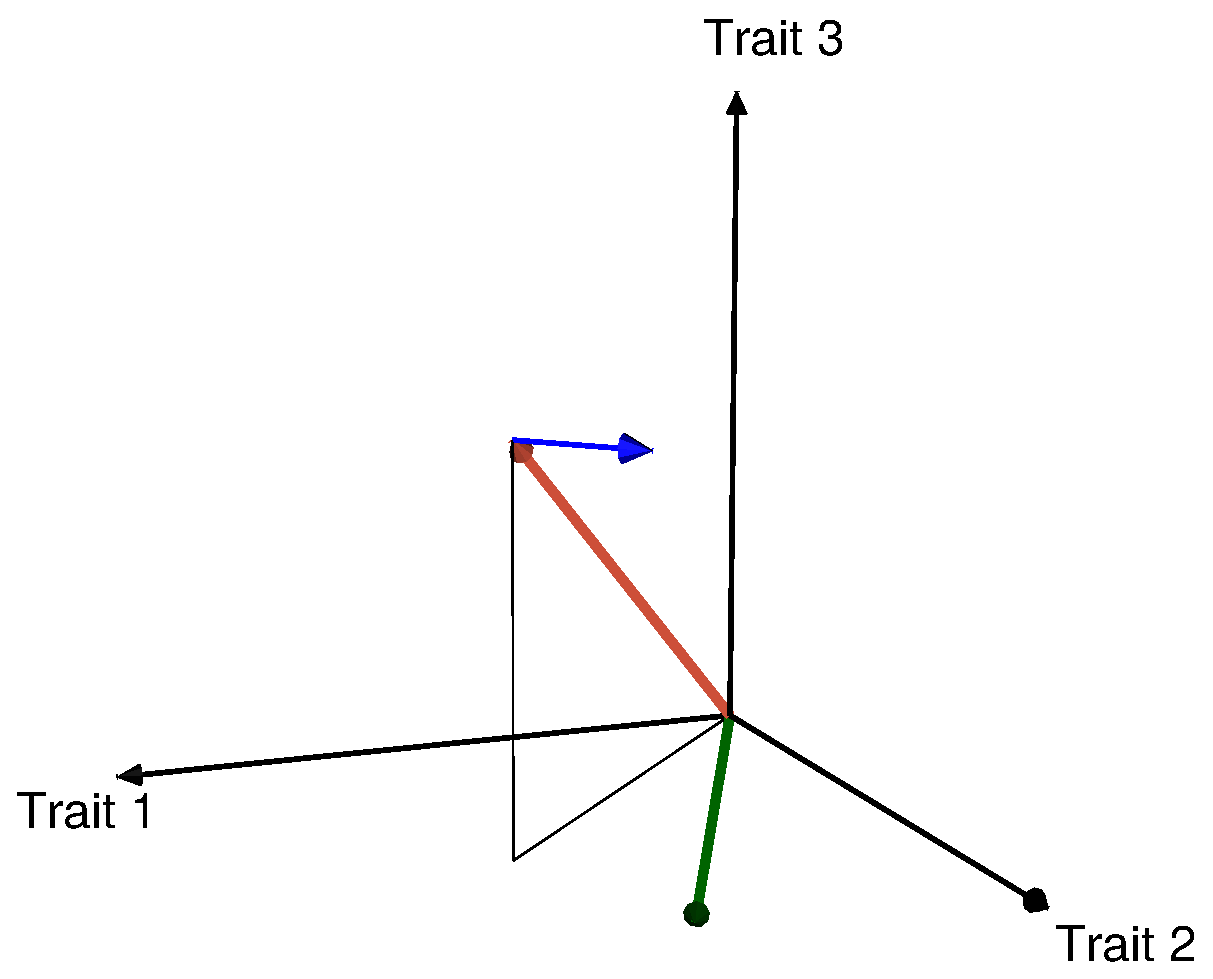
\includegraphics[width=\linewidth]{chapter_atchley/media/plot.eps}
    \caption[Pleiotropic effect in trait space]{Representation of vectors of genetic effects in trait space. Red vector is an integrative vector, while the green vector is modular with respect to traits 1 and 2. Blue vector represents a possible mutation that alters the direction of the red effect.}
    \label{effectvectors}
\end{figure}

\begin{figure}
    \centering
    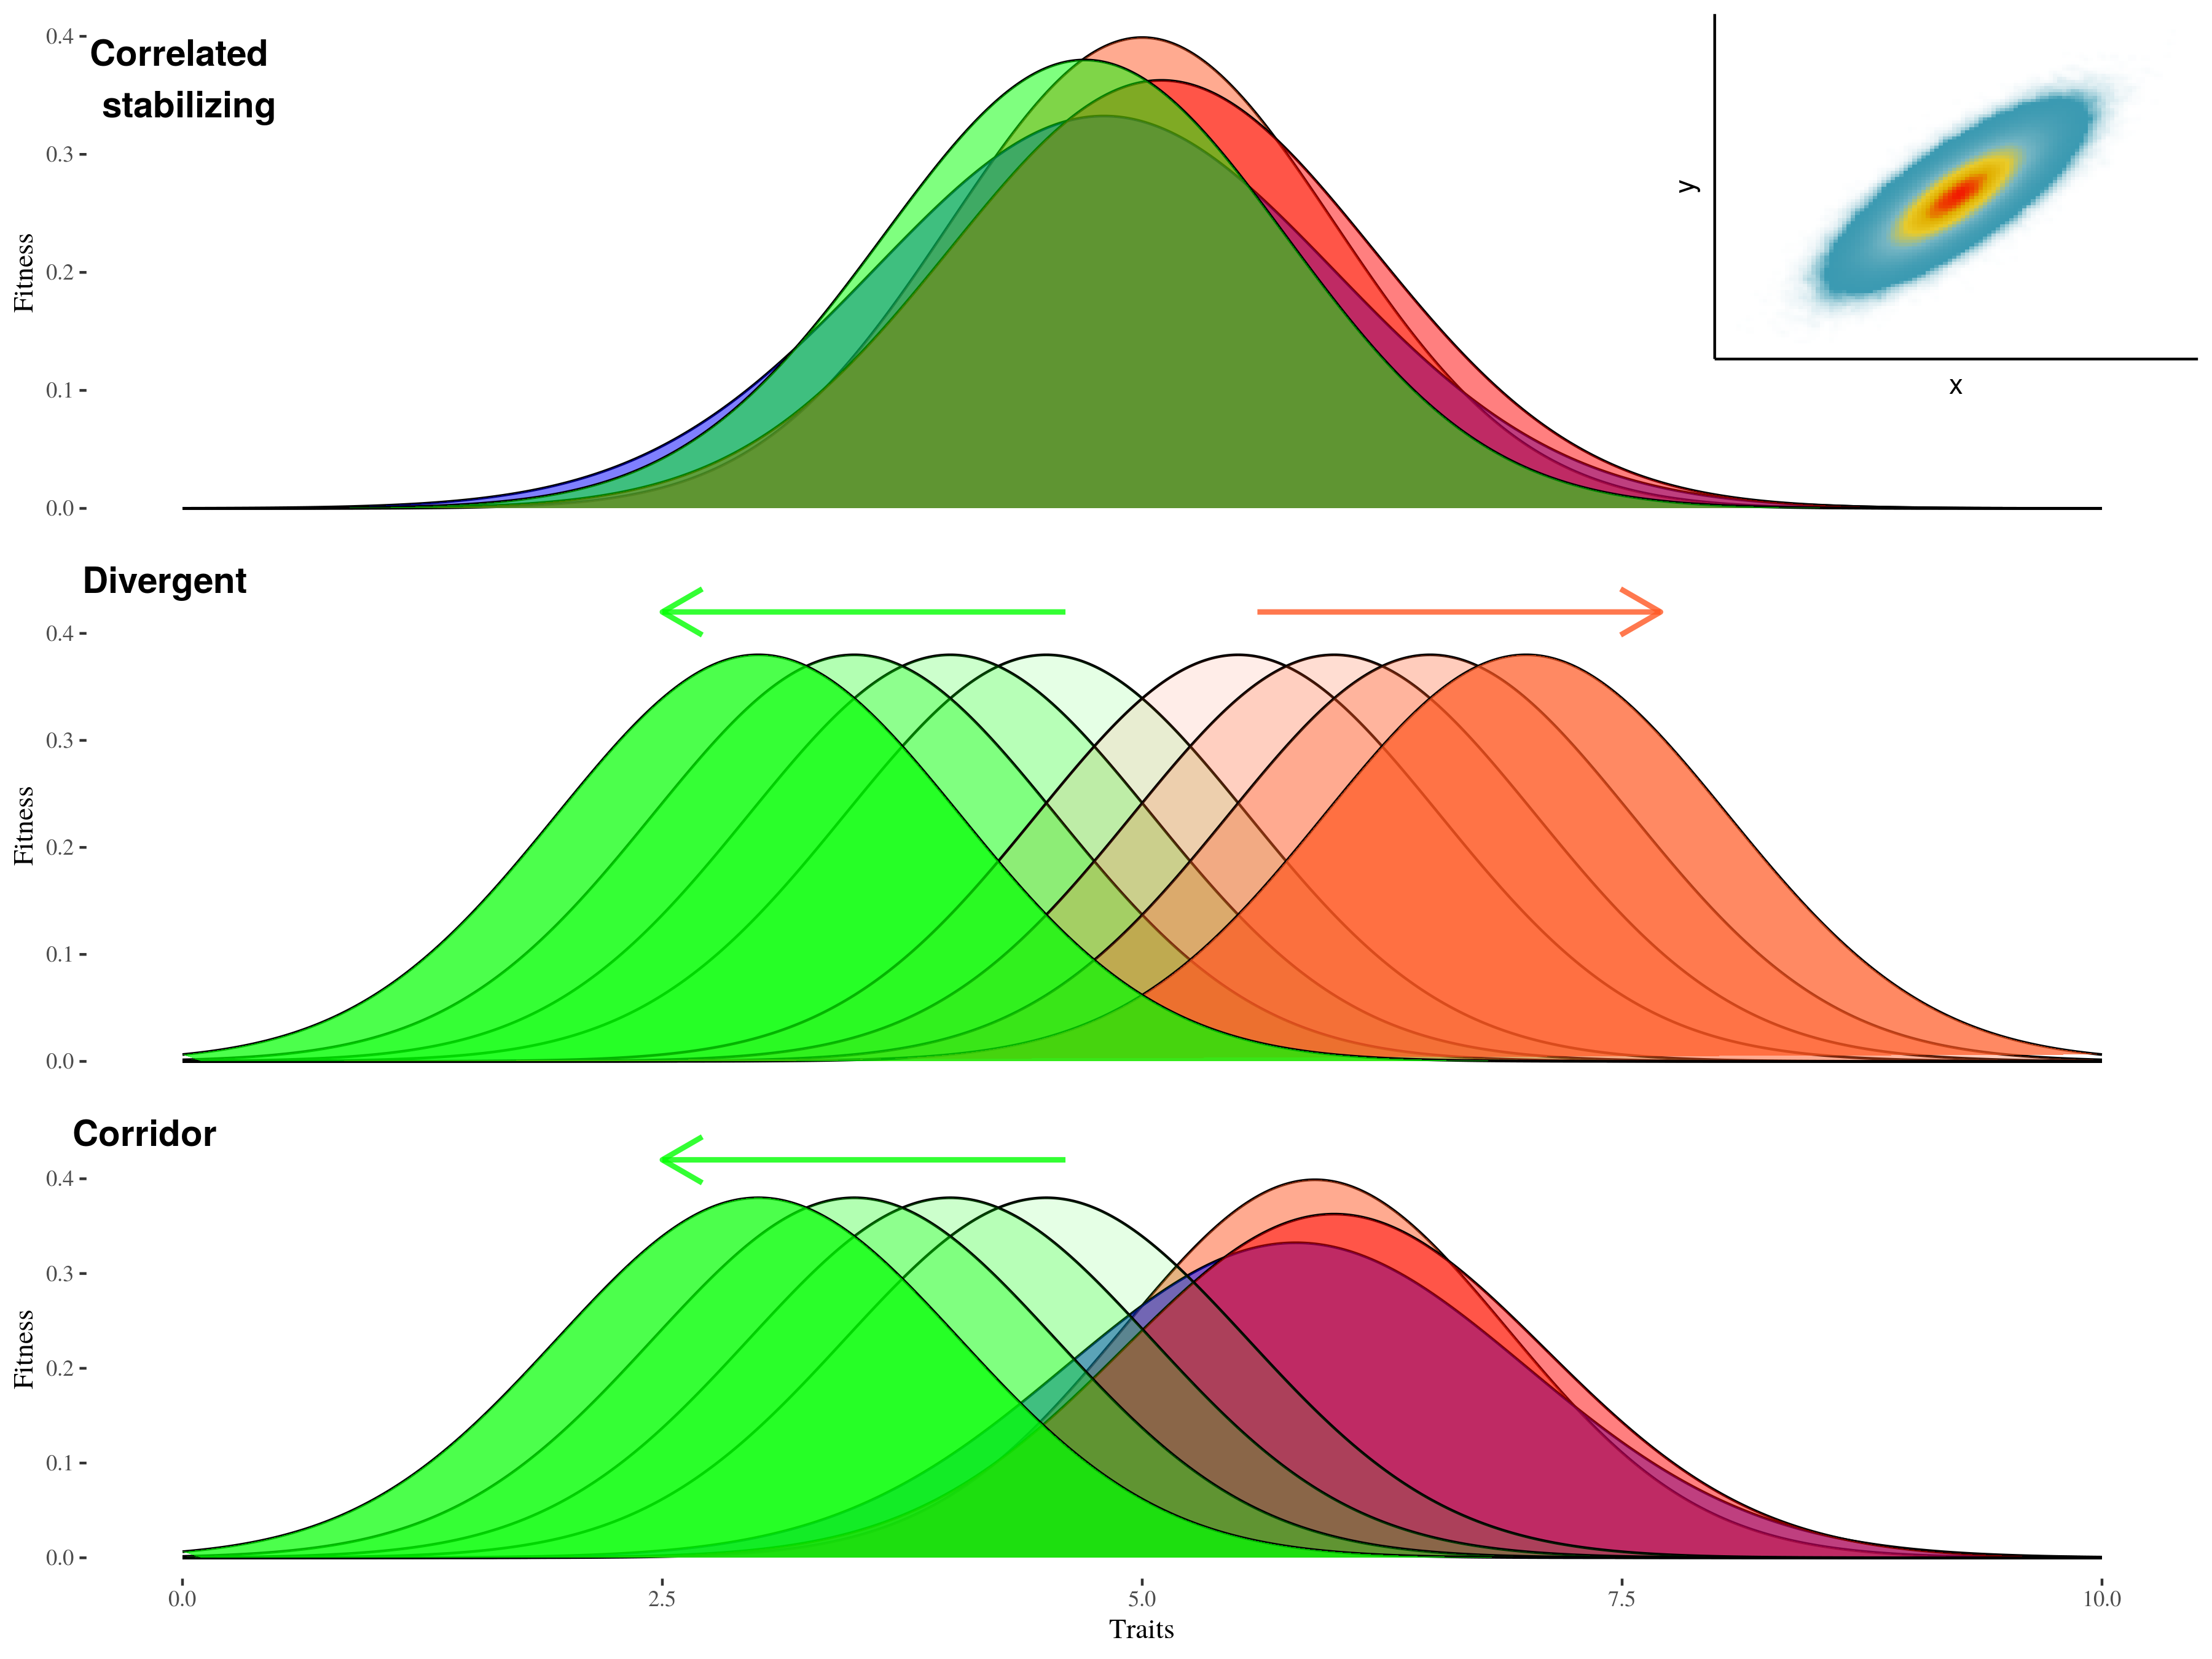
\includegraphics[width=\linewidth]{chapter_atchley/media/selection_types.png}
    \caption[Simulated selection regimes]{Representation of selection regimes.}
    \label{selectionregimes}
\end{figure}

\subsection{Mouse lines and phenotypes}

\subsubsection{Inbred strains} 
\label{ibs}

We founded our intercross population using inbred strains derived from a directional selection experiment by~\textcite{Atchley1997-vn}, in which each strain was selected for increase or decrease in their early (0 to 10 days) and late (28 to 56 days) growth rate, with corresponding compensatory selection in the other direction. For example, the E+ selection strain corresponds to an increase in early growth combined with a decrease in late growth. One of our six strains had been selected for fast early growth (E+, A13 strain), two for slow early growth (E-, A22 and A23 strains), one for fast late growth (L+, A31 strain), and two for slow late growth (L-, A41 and A42 strains).  After the selection regime, the strains were inbred for several generations, and were all <1\% heterozygous. Unfortunately, during the several years in which the selected strains were kept in an inbreeding regime, a mistake in the labeling of the animals during a move for a new mice facility led to a contamination of one of the E- strain (A22) with animals from one of the L- (A42) and the other E- strain (A23). This contamination caused an increase in the heterozigocity in the A22 line and some regions of the genome where that are only five segregating haplotypes instead of the expected six. We discuss this contamination further in the genotyping section. 

\subsubsection{Breeding scheme}

The six inbred strains were crossed non-reciprocally in every pairwise combination, giving 15 combinations in total. For three of the strains, 3 males and 2 females were used in crosses, each paired with a female or male from one of the other strains. For the other three strains, the reverse was true. This design gives an even balance of all six strains on the autosomes, and close to an even balance of the strains on the Y-chromosome and the mitochondria.
From the F1, two males and two females from each of the 15 litters were used in mating pairs, giving 30 combinations in total. The crossing scheme was designed such that there was no overlap in the strains that had been crossed to produce the parents in the previous generation. That is, each cross resulted in offspring that were a mixture of four of the strains.  Furthermore, the two males from a given litter were mated to females that themselves differed in both of the strains that had been combined to produce them.  This maximized the number of different strain combinations, and ensured representation of all six strains continued to be equal in the next generation.  All crosses were reciprocal in this generation (i.e. if a male from litter 1 was mated to a female from litter 2, then a male from litter 2 was mated to a female from litter 1). 
A version of this design that balances the contribution of each of the founder strains was continued up to the F4. However, each F2 mouse was a mixture of four of the six strains, therefore it was not possible to form pairs between unique strain combinations in this generation.  
To ensure all F3 mice included a contribution from all six strains, one male and one female from each of the F2 litters were used in non-reciprocal mating pairs, again giving 30 (unique) combinations in total, but pairs were chosen such that the parents overlapped in only two of the strains. This resulted in a double dose of two strains in each F3 offspring. To avoid unequal distribution of the strains in the population, we ensured there was an equal number of each pair of strains overlapping across the 30 pairs. 
For the F4 generation, one male and one female from each of the F3 litters were used in mating pairs, again giving 30 combinations in total. Each F3 mouse was a combination of all six strains, with a double dose of two strains. Pairs were chosen such that the male and female did not overlap in the strains they had a double dose of (i.e. all F4 offspring ended up with a deficiency of two strains).  To avoid unequal distribution of the strains in the population, we ensured there were equal numbers of litters deficient in each pairwise combination of strains.  All crosses were non-reciprocal.  One pair failed to produce any offspring, resulting in a very slight imbalance in the representation of the strains. 
For generation F5 and F6, matting pairs were combined at random, but avoiding within-litter mating and excluding duplicate litter combinations. Two males and two females from each F4 litter were used in mating pairs, giving 58 combinations (due to one F3 pair failing to produce a litter). Finally, three males and three females from each F5 litter were used in mating pairs, giving 174 unique litter combinations. On the day of birth, F6 litters were trimmed to a maximum of 10 pups (5 males, 5 females or as close to an even sex ratio as was possible given the numbers born).  All litters were cross-fostered between mothers within the breeding scheme within 2 days of birth (usually on the day of birth, but occasionally later if a foster mother was not available).  Thus, each female acted as a birth mother and a foster mother, and each litter was reared by a different mother to the one that gave birth to it. In total, we use 1513 animals from the F6 generation.

\subsubsection{Phenotypes}

All mice were weighed on the day of birth, then at 3 days, 7 days and then weekly until they were 8 weeks old. To define a low dimensional phenotype related to growth, we used the difference in weight over 2 weeks. So our analyses focus on weight gained over each two week interval (`growth') from one week to
eight weeks of age. These growth traits were calculated as the difference in body weight between the weeks that define each time interval (e.g., growth from birth to week 2 is defined as growth\textsubscript{0--2} = weight\textsubscript{2}
- weight\textsubscript{0})
 
\subsubsection{Genotypes}

The genomic data was extracted from the spleens of one mouse for each of the inbred strains. Each strain was then run in each lane of a flow cell and sequencing was conducted using paired end Illumina sequencing. This produced approximately 487 million total bases for each sample, all of 125bp in length. Galaxy \parencite{Goecks2010-hz} was used to conduct quantity control using FastQC on the untrimmed sequences. The sequence reads were trimmed in trimmomatic \parencite{Bolger2014-ra} using the following parameters: Cropped first 10 bases from each read, trimmed specified adapter sequences, allowed a maximum of 2 mismatches between the adapter and read sequence, palindrome Clip Threshold of 30, simple Clip Threshold of 10, minimum length of adapter detected of 8 bases, and retaining the reverse read to maintain pairing (\texttt{keepBothReads=true}). Following the trimming, we removed leading and trailing bases from reads with quality less than 3 using a sliding window of 4 bases and trimmed if mean quality was less than 15. The trimmed transcripts were then paired and aligned to mouse reference genome (mm10) using Bowtie 2 \parencite{Langmead2012-ev}. The \texttt{‘Local, sensitive’} alignment algorithm was used, with all other parameters left unchanged. After alignment, SNP calling was carried out using SAMtools \parencite{Li2009-yr} against the mm10 reference genome. The tool \texttt{‘Pileup’} was used to identify SNPs, with  parameters set to default. From this set of SNPs we set out to design a custom SNP array for genotyping in the intercross generations. Our initial strategy for designing the SNP genotyping array was to select private SNPs for all the strains along the genome. Private SNPs are SNPs that are biallelic among the founder strains, with one strain having one allele and the other five strains sharing the alternate allele. If the density of private alleles is high enough, this provides a trivial way of identifying the strain of origin of a particular stretch of the genome in the intercross line. However, the labeling mistakes in the maintenance of the inbred strains (described in section \ref{ibs}-\textbf{Inbred Strains}) caused some degree of interbreeding between some of the strains. This made selecting the SNPs for the genotyping array a more challenging task, since in some regions of the genome some of the strains lacked private alleles that would lead to the most informative SNP choice. Given this problem, we developed piecewise approach to select, in each segment of the genome, the most informative set of SNPs available. We divided the full genome into equal sized chunks, and in each chunk ranked the SNPs in terms of their information content: first private alleles (5:1 split of the strains), then SNPs where one allele was shared between two of the strains (4:2 splits) and finally SNPs where one allele was shared between three of the strains and the other between the other three strains (3:3 splits). We classified the SNPs into these broad groups, and then classified them into categories using the strains involved in the splits, so, we have 6 types of 5:1 SNPs, 15 types of 4:2 splits, and 10 types of 3:3 splits. We then selected at most 4 SNPs for each of these 31 classes of SNPs, totaling at most 50 SNPs per chunk. Selection for the SNPs in the same class was done by selecting the most high quality SNPs (as ranked by SAMtools). This resulted in a set of around 50000 SNPs with maximal information for each chunk that were used by Affymetrix to produce a custom SNP array\footnote{Fast parallel code for performing this SNP selection can be found in \url{https://github.com/diogro/EL-snp_selection}}. Using this array, we scored 55338 SNPs, of which 43934 were polymorphic in the intercross. These SNPs were scored in 2299 samples divided among the inbred parental strains, the F1, F5 and F6 generation. Quality control was done using the Affymetrix´s \textsc{Axiom Genotyping Solution: Data Analysis Guide}\footnote{\url{https://tools.thermofisher.com/content/sfs/manuals/axiom_genotyping_solution_analysis_guide.pdf}, last viewed in September 20th, 2018}. Samples with call rate below 97\% were discarded, resulting in 2243 samples. SNP quality control was done using Axiom Analysis Suite\footnote{\url{https://www.thermofisher.com/us/en/home/life-science/microarray-analysis/microarray-analysis-instruments-software-services/microarray-analysis-software/axiom-analysis-suite.html}, last viewed in September 20th, 2018}, and after standard quality control filtering we arrived at a final set of 33300 high quality biallelic SNPs distributed along the genome. These SNPs were scored in 1513 individuals from the F6 generation, 629 from the f5, 50 from the F1, e 26 parental individuals from the inbred strains. Phasing and imputation of missing SNP calls was done in Beagle 4.0 \parencite{Browning2007-el}, using the parent-offspring relations among the individuals to inform the imputation.

\subsection{QTL mapping}

In order to link genetic and phenotypic variation, we use 

\subsection{Genetic effect classification}


We can classify genetic effects on multiple traits by the sign of the effects on each of the traits in relation to a modularity hypothesis. For example, an allele that only increases two traits in the same module is defined as modular, while one effect that increases the traits in one module while decreasing the traits in a different module is antagonistic. We give some examples for four traits below, assuming traits [1,2] and [3,4] form modules.

\begin{figure}
    \centering
    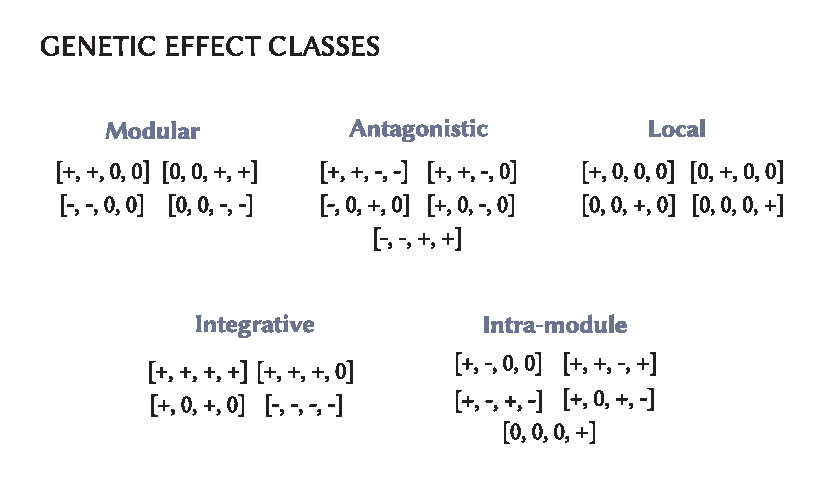
\includegraphics[width=\linewidth]{chapter_atchley/media/genetic_effects.eps}
    \caption[Pleiotropic vector classification]{Pleiotropic genetic effect can be classified according to the direction of the effect on multiple traits with regards to a modularity hypothesis. For example, modular allelic effects can be defined as those that change two or more traits in a module in the same direction, while having no effect in traits outside that module. We also define antagonistic effects as those that have effects in two or more modules in opposite directions, i.e. increasing module 1 while decreasing module 2. Local effects affect only one trait, integrative effects affect two of more modules in the same direction, and finally intra-module effects affect traits in opposite directions inside the proposed modular structure. A non-comprehensive set of examples is shown in the figure assuming a four trait two module .}
    \label{effectclassification}
\end{figure}


\printbibliography

\end{refsection}